\chapter{Evaluation}
\label{c:evalu}

In this chapter, we present the end-to-end evaluation of our system.
At first, we discuss the evaluation datasets and ground truth annotation.
Next, we present the quantitative results for both computation time and accuracy.
Finally, we conclude this chapter with evaluation of our system using a public dataset.

\section{Evaluation datasets}
\label{s:eval}
To our best knowledge, there is not much research on sensor fusion in the context of traffic light detection, especially for pedestrian navigation. 
As a result, we did not find public datasets combining traffic lights video and inertial sensor data. 
Hence, we collected our own ground truth data using an Android app \todo{refer section or fig with the screenshot}.
We walked across several street crossings and recorded both video and sensor data simultaneously in various lighting conditions. 
For example, \ref{f:dataset} shows video frames for both sunny and cloudy days. 
Here, we present our results for several 300 feet long walks.  
At the end of this chapter, we present an approximate evaluation of a public dataset that does not have sensor data. 
However, we emulate the effect of sensors by manual selection of a subpart of a video frame. 

\begin{figure}[!ht]
\centering
\subfloat[Sunny] {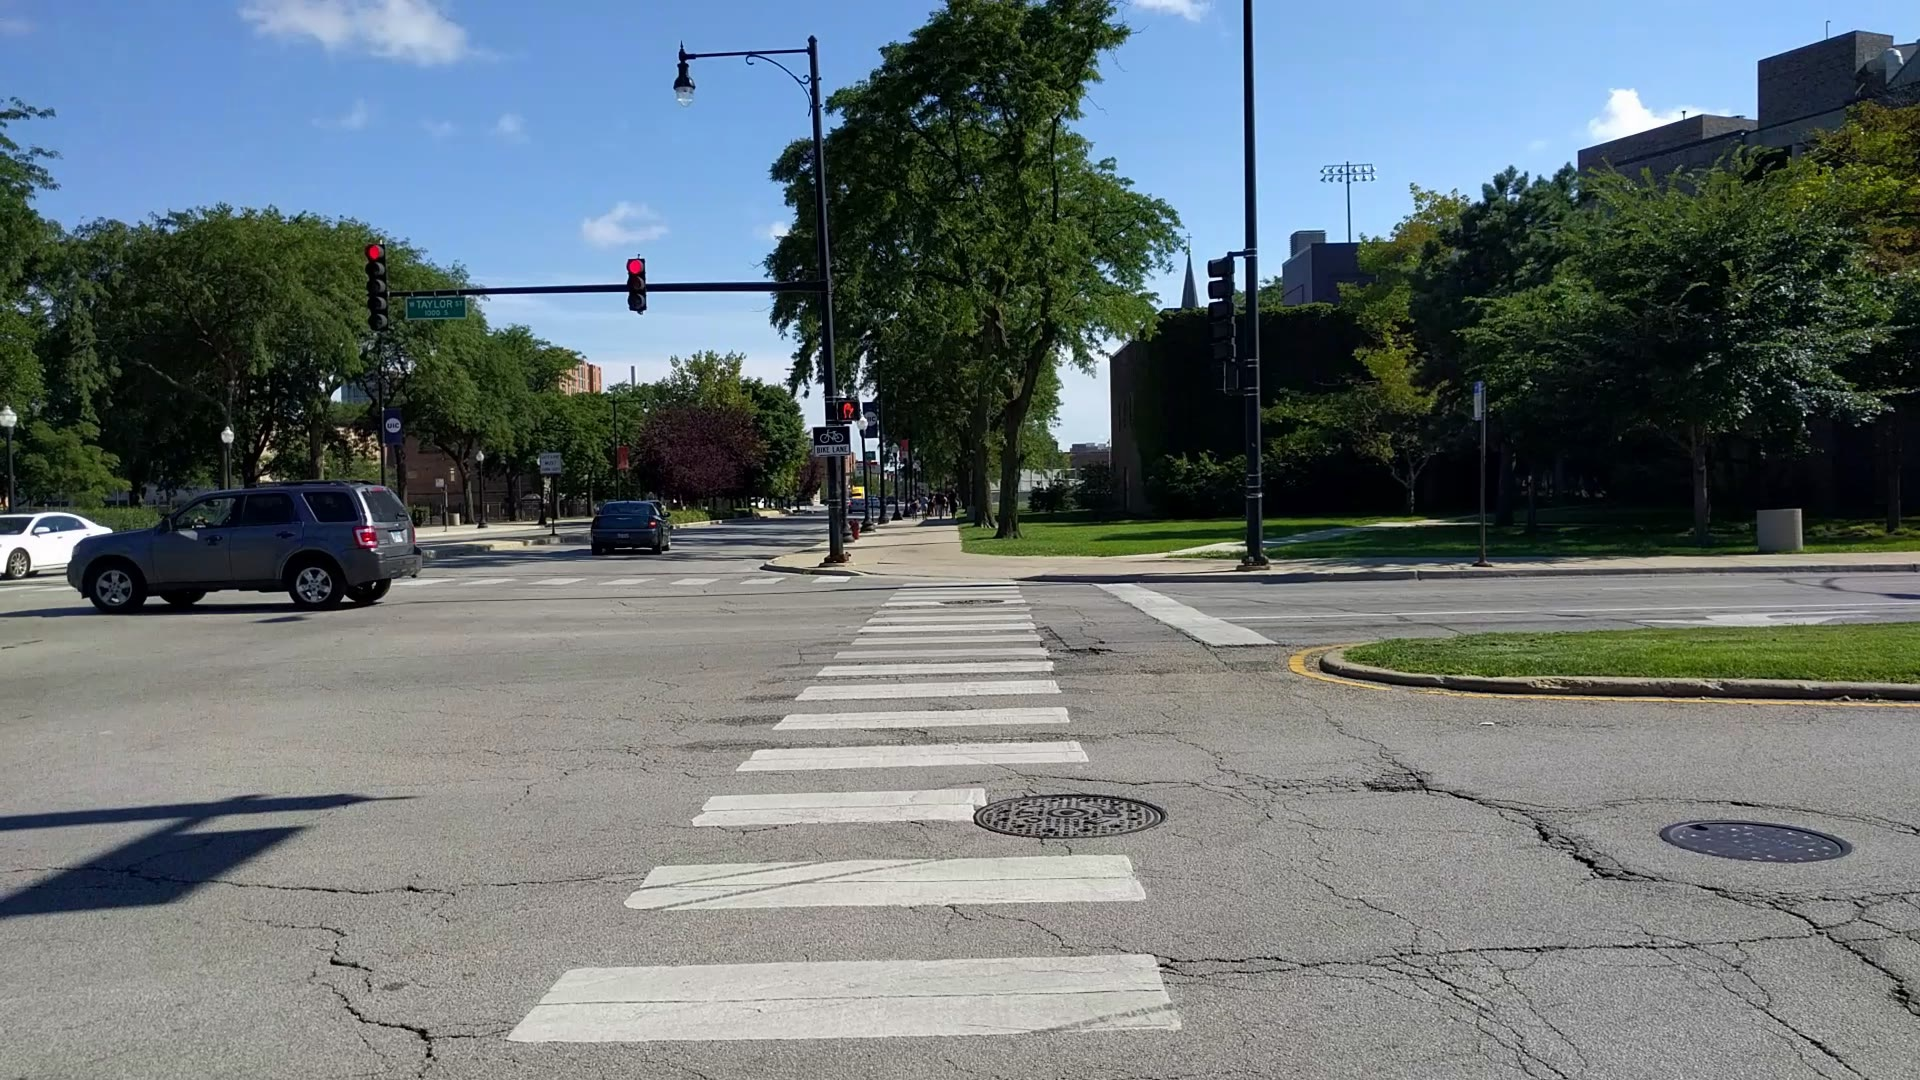
\includegraphics[width=3.1in]{images/sunny.jpg}}
\hfill
\subfloat[Cloudy] {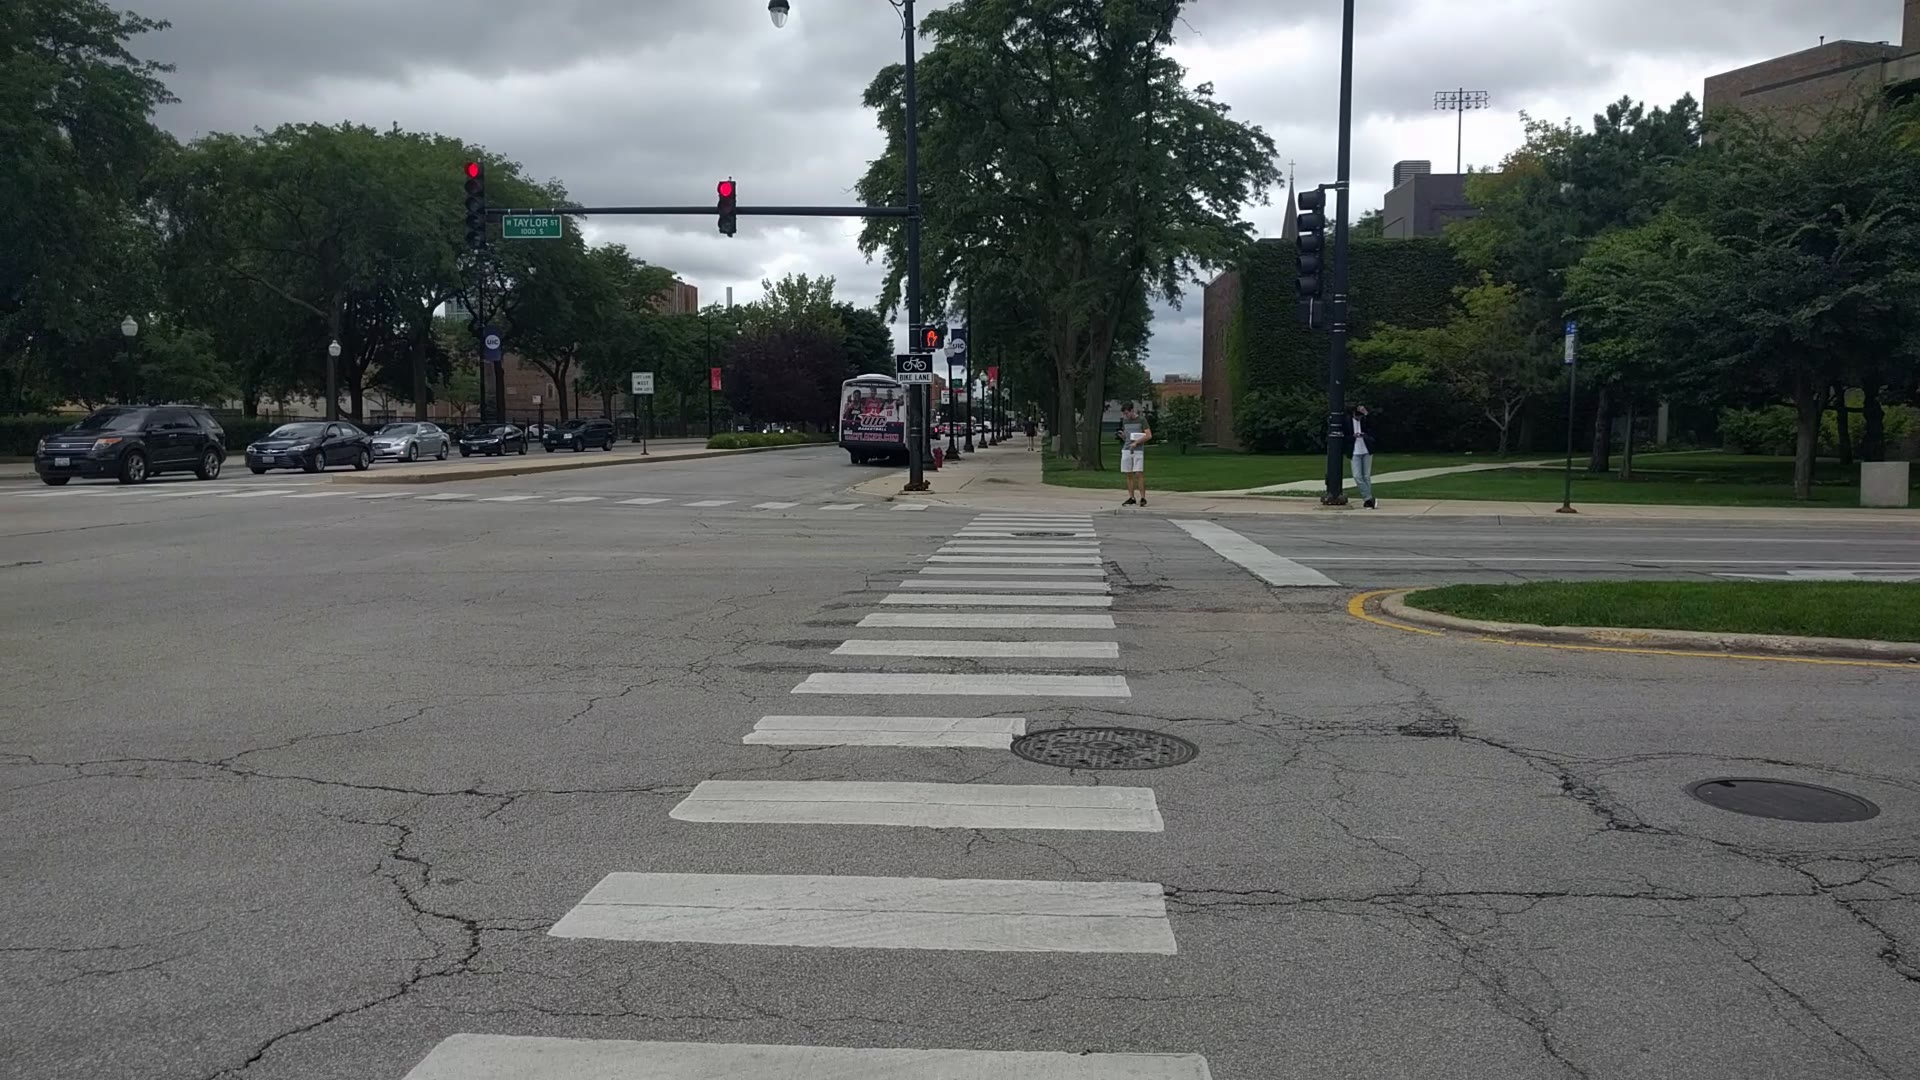
\includegraphics[width=3.1in]{images/cloudy.jpg}}
\caption{Scene variation of recorded video.}
\label{f:dataset}
\end{figure}

\ref{t:dataset} shows the total no of frames and time duration of our dataset.

\begin{table}[h!]
  \centering
  \caption{Description of the dataset.}
  \label{t:dataset}
  \begin{tabular}{  l  c  r  }
   
    Name & Frame Count & Time Duration \\
    \hline
    Walk with sensor movement-Sunny day & 5905 & 3 mins 16 secs  \\
    Walk with sensor movement-Cloudy day & 6205 & 3 mins 26 secs \\
    Walk regular movement & 6022 & 3 mins 20 secs \\
    Static with sensor movement & 1810 & 1 min \\
    \hline
  \end{tabular}
\end{table}

\section{Annotation}
We need the ground truth for traffic light positions on video frames in order to measure our system performance quantitatively.
Accordingly, we annotate the traffic light's positions manually by drawing a rectangle around the traffic lights at each video frame.
During annotation, we record the type of the traffic lights (i.e., red or green) and their positions with a bounding box.

\ref{f:annotate} shows the interface for manual annotation.
The green box provides the location of the traffic light and we annotate 0 for a red traffic light and 1 for a green traffic light.

\begin{figure}[h!]
\centering
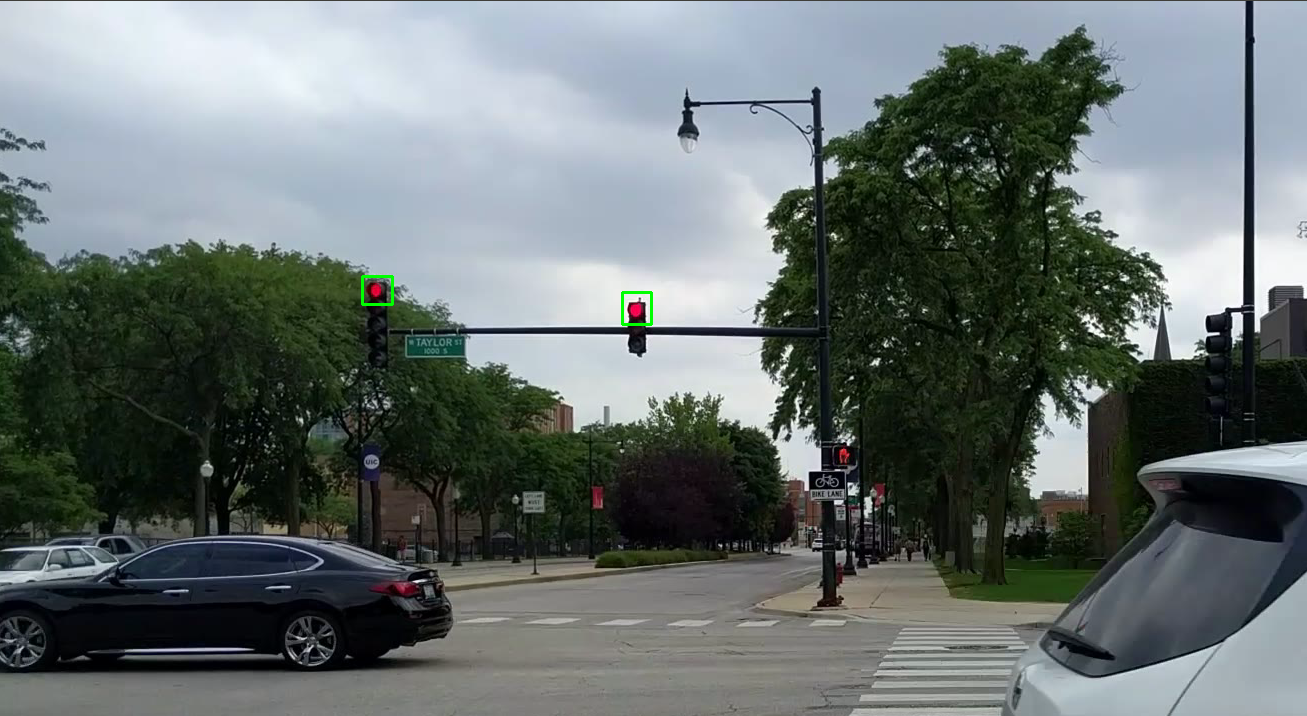
\includegraphics[width=5.2in]{images/annotation.png}
\caption{Interface for manual annotation.}
\label{f:annotate}
\end{figure}


\section{Computation time}
We collected data at different times of the day as we discussed in \ref{s:eval}.
In this section, we discuss the computation time of these datasets with and without the sensor fusion.

\subsection{Frame processing time}
\ref{f:cdf_time} shows the computation time CDF for video frames for walking dataset with regular movement described in \ref{t:dataset}.
It shows that the median of the computation time without the sensor data and without the heuristic filters is 106ms.
On the other hand, the median computation time with the sensor and without heuristic filters is 13ms.
This is an improvement of 8.15x.
The median computation time with sensor and heuristic filters is 19ms.
There is a slight increase in frame processing time with the heuristic filters, but this is worthwhile as we false detection rate reduces significantly with the heuristic filters.  
We discuss more about the accuracy and false detections in Section \ref{s:acc}

\begin{figure}[h!]
\centering
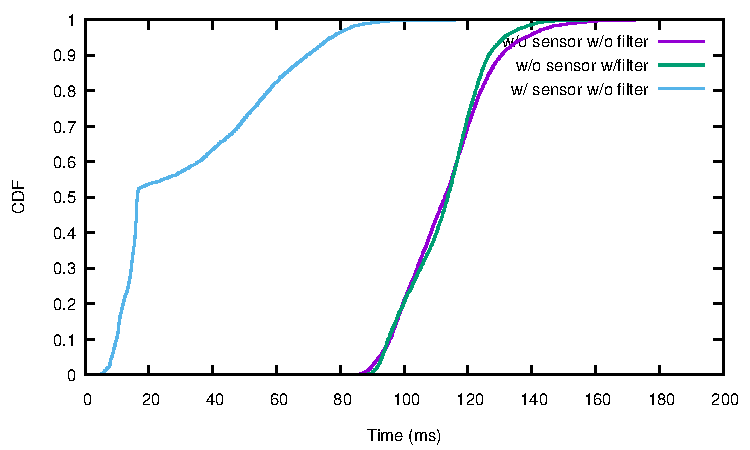
\includegraphics[width=5.2in]{plots/sunny_cdf_time.pdf}
\caption{CDF of frame computation time for walking dataset in sunny weather.}
\label{f:cdf_sunny}
\end{figure}

\ref{f:cdf_sunny} shows the CDF of the video frame computation time for walking dataset with sensor fusion on a sunny day.
It shows that the median computation time without the sensor is 107ms and with the sensor is 13ms, resulting in an improvement of 8.23x.


\subsection{Subimage processing time}
Processing a subpart of a video frame significantly reduces the computation time. 
We select a Region-Of-Interest (ROI) area within a frame with the sensor hints.
However, the ROI predicted from the sensor hints can be incorrect and we gradually increase the area of the rectangle.
We discussed the details about this in \ref{s:roi}.


\ref{f:recarea} shows the computation time with the increase of the ROI area in video frames.
It shows that the computation time increases as the area of the rectangle get larger.
For the same area, if the number of candidate pixels is high or the detected circle count is high then computation time can be also high.

\begin{figure}[h!]
\centering
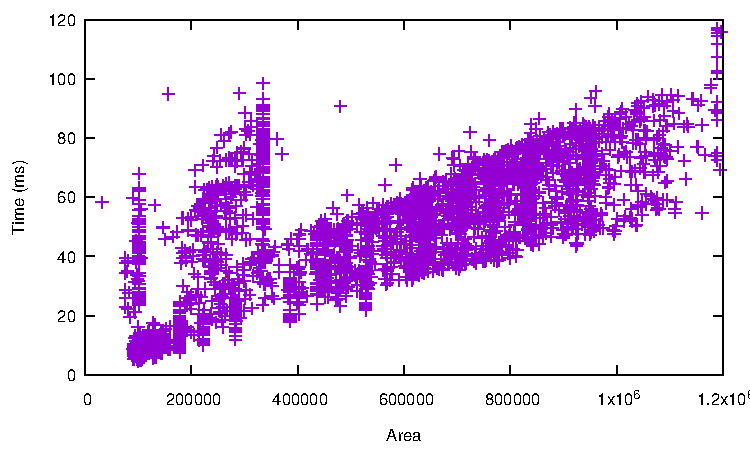
\includegraphics[width=5.2in]{plots/sunny_recarea.pdf}
\caption{Computation time with the increase of the rectangle area.}
\label{f:recarea}
\end{figure}



\subsection{Time for heuristic filtering}
We use a heuristic filter to reduce false positive in traffic light detection as we discuss at \S\ref{s:filter}.
The computational cost of the heuristic filter is very small.

\begin{figure}[h!]
\centering
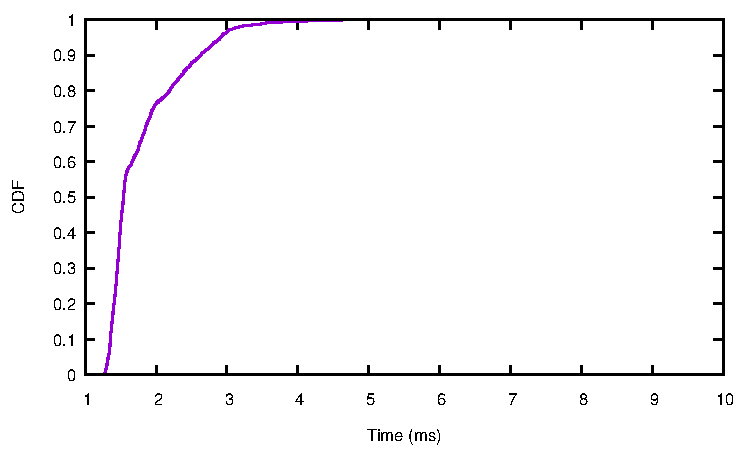
\includegraphics[width=5.2in]{plots/sunny_cdf_filter.pdf}
\caption{CDF of computation time for the heuristic filter.}
\label{f:cdf_fil}
\end{figure}

\ref{f:cdf_fil} shows the computation time of the heuristic filter that we discuss at \S\ref{s:filter}.
The computation time depends on the number of circles detected on the frame.
If circle count is high, filtering need for all of these circles, so computation time gets higher.
\ref{f:cdf_fil} shows that the median computation time is 1.5 ms for the filtering. 


\begin{figure}[h!]
\centering
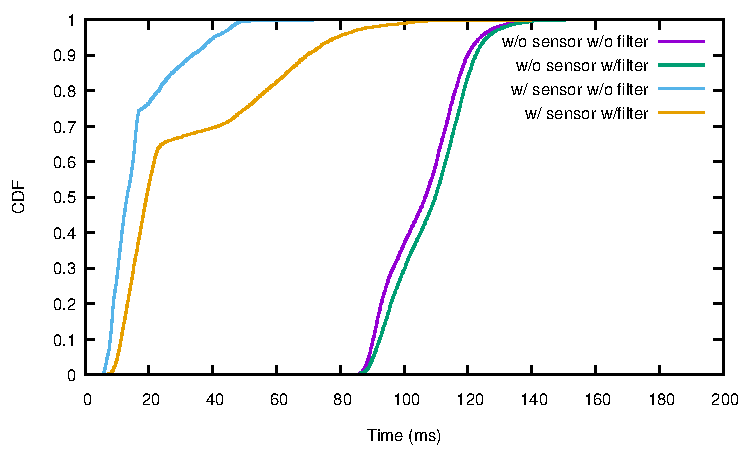
\includegraphics[width=5.2in]{plots/walk_cdf_time.pdf}
\caption{CDF of frame computation time.}
\label{f:cdf_time}
\end{figure}



\section{Traffic lights detection accuracy}
\label{s:acc}
To demonstrate the robustness of the various traffic light scenarios, we recorded video at different lightening condition such as cloudy and sunny and at the different time of the day.
We walked along several crosswalks of few streets and the route had a total of 16 traffic lights.

\subsection{Confusion matrix}
\ref{t:con_nocrp} shows the confusion matrix for the traffic light decision when we do not consider the sensor hints of the smartphone.
\ref{t:con_crp} shows the confusion matrix considering the sensor hints in the same dataset.

\begin{table}[h!]
  \centering
  \caption{Confusion Matrix without sensor hints for static movement dataset.}
  \label{t:con_nocrp}
  \begin{tabular}{  l | c | c | r }
   
     & Detected Red & Detected Green &  \\
    \hline
    Actual Red & 828 & 1 & 99.88\% \\
    \hline
    Actual Green & 54 & 509 & 90.41\% \\
    \hline
    & 93.88\% & 98.8\% & 96.05\% \\
    
  \end{tabular}
\end{table}

\begin{table}[h!]
  \centering
  \caption{Confusion Matrix with sensor hints for static movement dataset.}
  \label{t:con_crp}
  \begin{tabular}{  l | c | c | r }
   
     & Detected Red & Detected Green &  \\
    \hline
    Actual Red & 909 & 1 & 99.89\% \\
    \hline
    Actual Green & 36 & 524 & 93.57\% \\
    \hline
    & 96.19\% & 99.81\% & 97.48\% \\
    
  \end{tabular}
\end{table}

These results show that the use of sensor hints increases the accuracy of the red light detection and reduces false detection of green lights.


\subsection{Detection and misdetection rate for traffic lights}
\ref{f:tp_stat} shows the detection rate for the red and green state of the traffic lights.
It shows that using the sensor hints detection rate for red lights increases from 86\% to 96\% and the detection rate for green lights increases 96\% to 99\%.

\begin{figure}[h!]
\centering
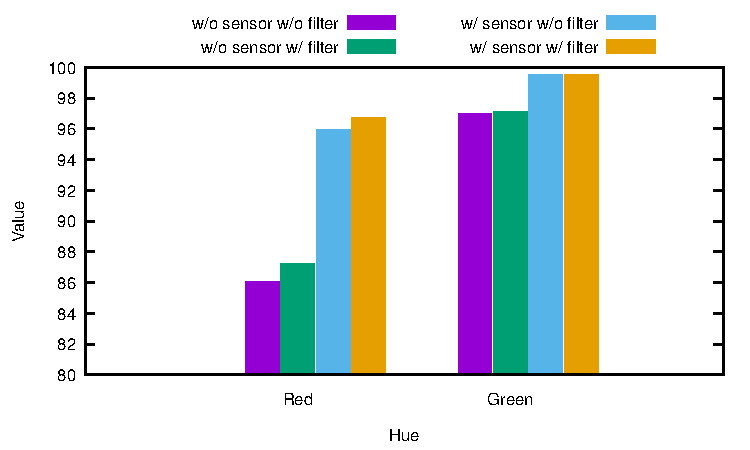
\includegraphics[width=5.2in]{plots/bar_tp.pdf}
\caption{Detection rate for static movement dataset.}
\label{f:tp_stat}
\end{figure}

\ref{f:fp_stat} shows the misdetection rate for the red and green state of traffic lights.
Left one is the false positive detection and the right one is the false negative detection for the traffic light detection.
Here, the false positive count is reduced significantly and false negative is zero.

\begin{figure}[!ht]
\centering
\subfloat[] {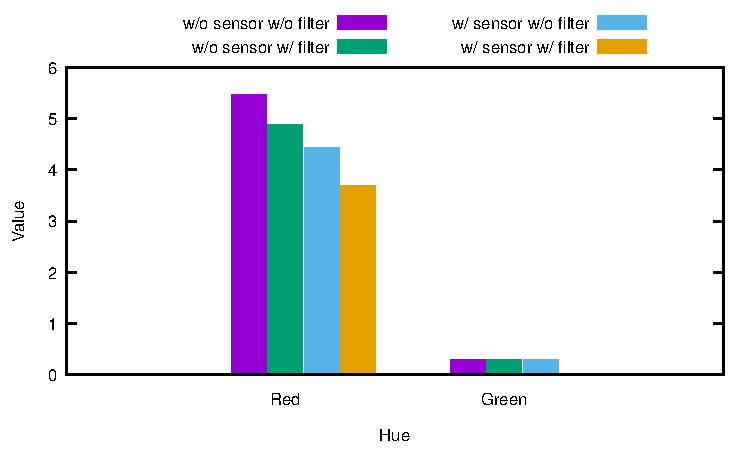
\includegraphics[width=5.2in]{plots/bar_fp.pdf}}

\subfloat[] {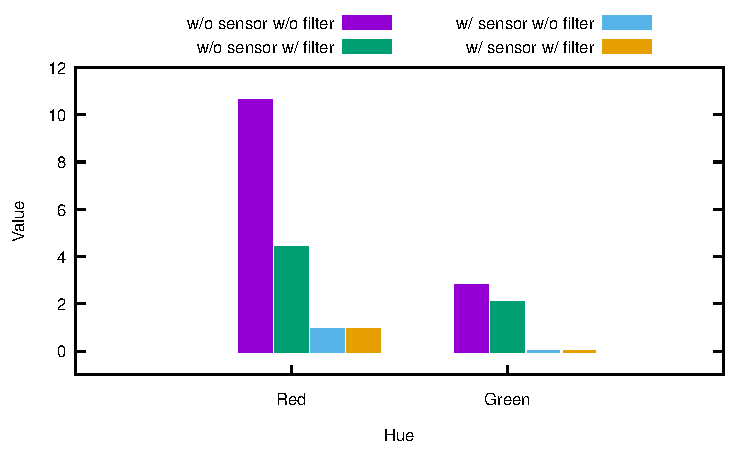
\includegraphics[width=5.2in]{plots/bar_fn.pdf}}
\caption{Misdetection rate for static movement dataset.}
\label{f:fp_stat}
\end{figure}

\ref{t:acc_stat} shows the accuracy rate for the static with sensor movement dataset.
It shows that the accuracy increases from 89\% to 97\% with sensor hints.

\begin{table}[h!]
  \centering
  \caption{Accuracy for detection.}
  \label{t:acc_stat}
  \begin{tabular}{  l  c | r  }
   
     & without sensor & with sensor  \\
    \hline
    & 89.7313\% & 97.035\%  \\
    \hline
  \end{tabular}
\end{table}


\section{Evaluation of a public dataset}

\todo{need to add results here}

\section{Effect of video/image resolution}

\todo{\ref{f:vf_res} shows the computation time after changing video frames resolution.}

\begin{figure}[h!]
  \centering
  \vspace{2in}
  %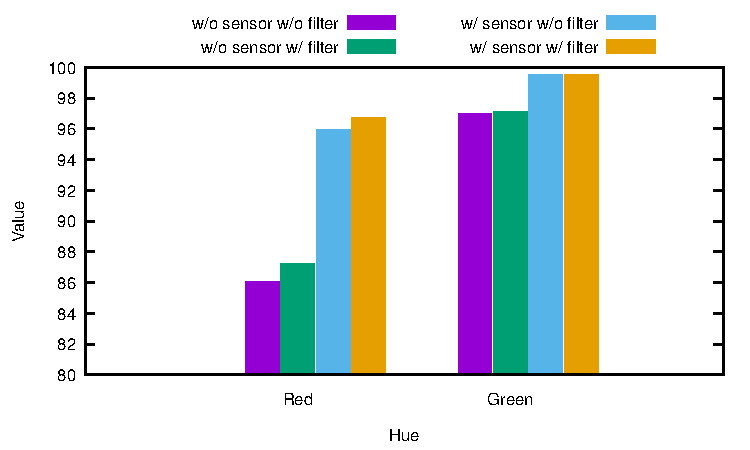
\includegraphics[width=5.2in]{plots/bar_tp.pdf}
  \caption{Effect of the computation time after changing video frames resolution.}
  \label{f:vf_res}
\end{figure}

